\cotefile{64}
\scanpage{116}
% archive foliation: 115
soit
\[
\tag{61}
\sigma_i z=\frac{\zeta_i z+\overbrace{\zeta_\lambda\zeta_\mu-\zeta_i(\zeta_\lambda+\zeta_\mu)}^{b_i}}{z-\zeta_i}.
\]
On peut transformer $b_i$ en utilisant les fonctions symétriques élémentaires $(-1)^\alpha a_\alpha$ des $\zeta$,
\[
b_i=2\underbrace{\zeta_\lambda\zeta_\mu}_{-a_3/\zeta_i}-\underbrace{(\zeta_i\zeta_\lambda+\zeta_\lambda\zeta_\mu+\zeta_\mu\zeta_i)}_{a_2}=-(a_2+2a_3/\zeta_i)
\]
donc on trouve
\[
\tag{62}
\sigma_i z=\frac{\zeta_i z-(a_2+2a_3/\zeta_i)}{z-\zeta_i}=\frac{\zeta_i^2z-(a_2\zeta_i+2a_3)}{\zeta_i z-\zeta_i^2}
\]
\margin{expressions valables du moins si $\zeta_i\ne0$, sinon on convient bien sûr que $a_3/\zeta_i$ \unsure{signifie} $\unsure{-}\zeta_\lambda\zeta_\mu$. Mais quitte à modifier \unsure{les $a_i$}, on \unsure{peut même supposer} les $\zeta_i\ne0$\ldots}
Les \inserted{div. $\Delta_i$ des} points fixes de $\sigma_i$ est l'ens. div. des solutions de l'équation en $z_i$
\[
\tag{63}
z_i^2-2\zeta_i z_i+(a_2+2a_3/\zeta_i)=0
\]
dont les solutions sont données par
\[
\tag{64}
z_i=\zeta_i\pm\sqrt{\underbrace{\zeta_i^2-a_2-2a_3/\zeta_i}_{\deleted{\unsure{\zeta}}}}
\]
L'expression sous le signe $\sqrt{\phantom{x}}$ s'écrit aussi
\[
\frac{1}{\zeta_i}(\zeta_i^3-a_2\zeta_i-2a_3)
\]
ou encore, compte tenu de (60)
\[
\zeta_i^3=-a_1\zeta_i^2-a_2\zeta_i-a_3
\]
\deleted{ce radical} cette expression devient
\[
-\frac{1}{\zeta_i}(a_1\zeta_i^2+2a_2\zeta_i+3a_3)
\]
donc (64) s'écrit aussi
\[
\tag{\textcircled{65}}
\left\{\begin{aligned}
(z_i-\zeta_i)^2&=-\frac{1}{\zeta_i}(a_1\zeta_i^2+2a_2\zeta_i+3a_3)\\
\text{i.e.}\quad z_i&=\zeta_i\pm\sqrt{-\frac{1}{\zeta_i}(a_1\zeta_i^2+2a_2\zeta_i+3a_3)}
\end{aligned}\right.
\]
\margin{Si $\zeta_i=0$, on \deleted{\unsure{peut écrire ainsi}} $-(a_1\zeta_i+2a_2+\unsure{3\zeta_\lambda\zeta_\mu|\zeta_\lambda\zeta_\mu})$ l'expr. sous le radical\ldots}
Les douze points d'ordre $4$ de $E$ sont donc les points au dessus des six points $z_i$, donc \deleted{définis par} \inserted{en tout}

\scanpage{117}
% archive foliation: 116
point est obtenu, pour un $i$ et un $z_i$ fixé, par le choix d'un $z'_i$ satisfaisant
\[
\tag{66}
{z'_i}^2=\underbrace{z_i^3+a_1z_i^2+a_2z_i+a_3}_{(z_i-\zeta_i)(z_i-\zeta_\lambda)(z_i-\zeta_\mu)}.
\]
Choisir, pour $\forall i\in\unsure{J|I}$, un $x_i\in E(k)$ tel que
\[
\tag{67}
2x_i=\varepsilon_i
\]
revient donc à choisir, pour $\forall i$, des quantités
\[
\tag{68a}
\wp(x_i)=z_i
\]
soumises à (65) \inserted{(2 choix possibles)}, et ensuite, la quantité $z'_i$
\[
\tag{68b}
\wp'(x_i)=z'_i,
\]
soumise à (66) --- ce qui fait quatre choix possibles pour $\forall i$, comme il se doit (car l'indétermination pour $x_i$ est dans $ {}_2E(k)$).

Ceci posé la condition d'épinglage de Jacobi relatif d'échelon $4$
\[
\tag{69}
\sum_{i\in\unsure{J|I}}x_i=0
\]
s'exprime par la condition
\[
\tag{70}
\left\{\begin{aligned}
\det\begin{pmatrix}
1&z_1&z'_1\\
1&z_2&z'_2\\
1&z_3&z'_3
\end{pmatrix}&=0\qquad\text{i.e.}\\
(z_1z'_2-z_2z'_1)+(z_2z'_3-z_3z'_2)+(z_3z'_1-z_1z'_3)&=0.
\end{aligned}\right.
\]
Cf prop. \unsure{3)}, qui s'applique, car les $x_i$ sont tous distincts. ---)

\scanpage{118}
% archive foliation: 117
En mettant ensemble les équations pertinentes :
\[
\tag{71}
\left\{\begin{aligned}
(z_i-\zeta_i)^2&=-\frac{1}{\zeta_i}(a_1\zeta_i^2+2a_2\zeta_i+3a_3)
\quad[=-(a_1\zeta_i+2a_2+3\zeta_\lambda\zeta_\mu)]\\
{z'_i}^2&=z_i^3+a_1z_i^2+a_2z_i+a_3
\quad[=(z_i-\zeta_i)(z_i-\zeta_\lambda)(z_i-\zeta_\mu)]\\
\det\begin{pmatrix}1&z_1&z'_1\\1&z_2&z'_2\\1&z_3&z'_3\end{pmatrix}&=0
\quad\text{i.e.}\quad
\underbrace{(z_2z'_3-z_3z'_2)}_{\psi_1}
+\underbrace{(z_3z'_1-z_1z'_3)}_{\psi_2}
+\underbrace{(z_1z'_2-z_2z'_1)}_{\psi_3}=0
\end{aligned}\right.
\]
\margin{$z_i^2=2\zeta_i z_i-(a_2+2\zeta_\lambda\zeta_\mu)\Longleftrightarrow$}
\margin{\uline{NB.} $[\psi_i^\omega=z_jz'_k-z_kz'_j,\quad j=\omega i,\ k=\omega^2i=\omega j]$}
qui expriment conjointement la donnée de $(x_i)_{i\in\unsure{J|I}}\in E(k)^{\unsure{J|I}}$ satisfaisant (67) (69),
\[
\tag{72}
2x_i=\varepsilon_i\ (\in{}_2E(k)^*),\quad \sum x_i=0
\]
via
\[
\tag{73}
z_i=\wp(x_i),\quad z'_i=\wp'(x_i).
\]

Je voudrais, à une telle donnée $(x_i)_{i\in\unsure{J|I}}$, exprimée calculatoirement (via le choix d'un $\delta\in\underline{t}_E^*$ et $\wp\in\unsure{F_2|\mathcal F_2}$ associés) par (71), associer \inserted{canoniquement} un \uline{épinglage de Legendre de $E$}, de façon fonctorielle en $E$ et compatible avec \unsure{les changements} de corps de base (entre autres). Je vais pour ceci supposer d'abord fixé un
\[
\tag{74}
\hat\imath\in\mu_4^*(k),
\]
de sorte que, via ce choix, la première donnée $\alpha$ d'un épinglage de Legendre de $E$ s'interprète comme un élément
\[
\tag{75}
\omega\in\underline{\omega}=\underline{\omega}_{\unsure{J|I}}
\qquad
\text{un ordre circulaire sur }J={}_2E(k)^*=\{\varepsilon_i\},
\]
\margin{$\alpha=\hat\imath\wedge\omega$}
de sorte que la deuxième donnée $\kappa$ s'interprète comme un isomorphisme :
\[
\tag{76}
\kappa:\underline{t}_E\xrightarrow{\sim}
\mathcal O_{\Sigma_J,t}(1)^{\unsure{\vee}}
\xrightarrow[\inserted{\text{grâce au choix de }\hat\imath}]{\sim}
\mathcal O_t(1),
\]

\scanpage{119}
% archive foliation: 118
satisfaisant à la condition que son carré $\kappa^{\unsure{\otimes2|\otimes}}$ s'\deleted{\unsure{se}}identifie, via les isom. canoniques
\[
\tag{77}
\underline{t}_E^{\unsure{\otimes2|\otimes}}\simeq T_{\Sigma_J,t},
\qquad
\mathcal O_t(1)^{\otimes2}=\mathcal O_t(2)
\underset{\text{via }\alpha}{\simeq}
\mathcal O_t(2)(\underline{\omega})\simeq T_{\Sigma_J,t}
\]
à l'isom identique de $T_{\Sigma_J,t}$ --- ce qui, pour $\alpha$ fixé (deux choix), détermine $\kappa$ modulo signe. Pour $\alpha$ non fixé, $\kappa$ est déterminé modulo multiplication par $\mu_4(k)$.

Rappelons-nous de la suite exacte canonique

(78)
\diagram{\begin{tikzcd}[ampersand replacement=\&,column sep=small]
0 \arrow[r] \& F_t \arrow[r] \arrow[d,"\wr" description,phantom] \&
V_J(k) \arrow[r] \arrow[d,"\wr" description,phantom] \&
\mathcal O_t(1) \arrow[r] \& 0\\
\& \mathcal O_t(-1)(\underline{\omega}) \&
\Gamma(\Sigma_J,\underline{\mathcal O}_{\Sigma_J}(1)) \&\&
\end{tikzcd}}

que \deleted{\unsure{pour faire}} je compare à

(79)
\diagram{\begin{tikzcd}[ampersand replacement=\&,column sep=small]
0 \arrow[r] \& k.1_{\Sigma_J} \arrow[r] \&
\overbrace{\Gamma(\Sigma_J,\underbrace{\underline{\mathcal O}_{\Sigma_J}\{t\}}_{\substack{\simeq\underline{\mathcal O}_{\Sigma_J}(1)\\\text{non canoniquement}}})}^{\simeq F_2}
\arrow[r] \& T_{\Sigma_J,t}\arrow[r] \& 0
\end{tikzcd}}

On constate que la deuxième suite exacte est canoniquement isom. à celle déduite de la première, en la tensorisant par
\[
\tag{80}
\check F_t\simeq\mathcal O_t(1)(\underline{\omega})
\]
(on a un iso valable chaque fois qu'on a un Module loc libre de rang $2$, $\underline V$, \deleted{\unsure{dont}} et une section $t$ de $\mathbb P(\underline V)$ \ldots) :

\deleted{(79)} (81)
\diagram{\begin{tikzcd}[ampersand replacement=\&,column sep=small]
0 \arrow[r,dash] \&
F_t\otimes\check F_t \arrow[r] \arrow[d,"\wr" description] \&
V_J(k)\otimes\check F_t \arrow[r] \arrow[d,"\wr" description] \&
\overbrace{\mathcal O_t(1)\otimes\check F_t}^{\underline{\mathcal O}_t(2)(\underline{\omega})} \arrow[r] \arrow[d,"\wr" description] \& 0\\
0 \arrow[r] \& k.1_{\Sigma_J}\arrow[r] \&
\underbrace{\Gamma(\Sigma_J,\underline{\mathcal O}_{\Sigma_J}\{t\})}_{F_2}
\arrow[r] \& T_{\Sigma_J,t}\arrow[r] \& 0 .
\end{tikzcd}}

\scanpage{120}
% archive foliation: 119
La donnée d'un isom $\kappa:\underline t_E\simeq\mathcal O_t(1)$ équivaut à celui de
\[
\check\kappa:\check{\underline t}_E\simeq
\underline{\mathcal O}_t(1)^\vee\simeq\underline{\mathcal O}_t(-1)
\xrightarrow{\text{via }\omega}
\underline{\mathcal O}_t(-1)(\underline{\omega})\xrightarrow{\sim}F_t
\]
ou encore, à celui d'un \deleted{ce qui \unsure{implique un épinglage}} monomorphisme
\diagram{\begin{tikzcd}[ampersand replacement=\&]
\check t_E\arrow[r,hook]\&V_J(k)\arrow[r,hook]\&k^J
\end{tikzcd}}
dont l'image soit $F_t$, ou enfin à celui d'un élément non nul de
\[
\deleted{\unsure{\delta}}\quad
V_J(\underline t_E)=\deleted{\unsure{\underline t_E^J}}\quad
\operatorname{Ker}(\underline t_E^J\xrightarrow[\text{somme}]{}\underline t_E)
\]
donc on peut considérer que la donnée de $\kappa$ revient à celle d'une famille
\[
\tag{82}
(\delta_i)_{i\in J}\in\underline t_E^J
\]
satisfaisant à certaines relations, savoir
\[
\tag{83}
\left\{\begin{array}{ll}
\text{a)}&\sum\delta_i=0\quad\text{exprimant }\delta_i\in V_J(\underline t_E)\\[3pt]
\text{b)}&\text{Relation de proportionnalité, exprimant que}\\
&\text{l'image de }\unsure{\check{\underline t}_E|\underline t_E}\hookrightarrow V_J(k)\text{ défini par }(\delta_i)\text{ est }F_t,\\
&\text{de sorte que }(\delta_i)\text{ définit }
\kappa:\underline t_E\xrightarrow{\sim}\check F_t
\underset{\text{via }\omega}{\simeq}\mathcal O_t(1)\\[3pt]
\text{c)}&\text{Relation de l'épinglage de Legendre, exprimant}\\
&\text{que }\kappa^{\otimes2}\text{ est un isom. }\unsure{\text{standart}|\text{standard}}\text{ déjà connu.}
\end{array}\right.
\]
Nous allons expliciter les $\delta_i$ en termes du choix d'un $\delta\in\underline t_E^*$, \inserted{en plus du choix de $\omega\in\underline\omega$,} comme
\[
\tag{84}
\delta_i=\varphi_i^\omega(\delta)\delta
\qquad
\begin{gathered}
\text{où }\varphi_i^\omega(\delta)\in k^*\\
(i\in J,\ \omega\in\underline\omega(J),\ \delta\in\underline t_E^*)
\end{gathered}
\]
La condition d'invariance de $\delta_i$ p.r. au choix de $\delta$ s'exprime par la relation
\[
\tag{85}
\varphi_i^\omega(\lambda\delta)=\frac1\lambda\varphi_i^\omega(\delta)
\]

\scanpage{121}
% archive foliation: 120
la condition (\unsure{83|82}) a) s'exprime par
\[
\tag{86}
\sum_i\varphi_i^\omega(\delta)=0
\]
la condition b) par la condition
\[
\tag{87}
k.((\varphi_i^\omega(\delta))_i)=F_t
\]
qui détermine d'emblée les $(\varphi_i^\omega(\delta))_i$ à scalaire inv. près --- la condition c les déterminant enfin (pour $\hat\imath$ également choisi) au \uline{signe} près.

Bien sûr, \deleted{on aura} \inserted{la relation entre $\kappa$ et les $\varphi_i^\omega(\delta)$ s'explicite par}
\[
\tag{88}
(\varphi_i^\omega(\delta))=
\underbrace{\check\kappa(\delta^\vee)}_{\mathcal O_t(-1)}
\wedge\omega
\in\mathcal O_t(-1)(\underline\omega)\simeq F_t\subset V_J(k)\subset k^J
\]
et la condition c) s'écrit Dieu sait comment --- il faudra \deleted{$\unsure{\varphi_i^\omega(\delta)}$} y revenir. Reste à exprimer la dépendance p.r. à $\omega$, pour \deleted{\unsure{exp}} trouver l'invariance de l'épinglage de Legendre p.r. au choix de $\hat\imath$ i.e. p.r. au choix de $\omega=\omega_{\hat\imath}$ ($\alpha:\mu_4^*(k)\simeq\underline\omega$ étant supposé déterminé), on trouve la relation nécessaire
\[
\tag{89}
\varphi_i^{\omega'}(\delta)=\deleted{\unsure{\imath_\omega^{-1}}}\imath_\omega\varphi_i^\omega(\delta)
\]
où
\[
\imath_\omega\overset{\text{déf}}=\alpha(\omega)
\qquad
\begin{gathered}
\alpha:\mu_4^*\simeq\underline\omega\ \text{étant l'iso.}\\
\text{(supposé déterminé)}\\
\text{associé à l'épinglage}\\
\text{de Legendre cherché}
\end{gathered}
\]

Posant

\scanpage{123}
% archive foliation: 122
\diagram{\begin{tikzcd}[ampersand replacement=\&,column sep=small]
\zeta_1\arrow[d,mapsto]\&\zeta_2\arrow[d,mapsto]\&\zeta_3\arrow[d,mapsto]\&{}\in k\&\&\infty\arrow[dll,bend right=20,mapsto]\\
0\&1\&\infty\&t\&\&
\end{tikzcd}}

\[
\left\{\begin{array}{l}\zeta_1,1\\\zeta_2,1\\\zeta_3,1\end{array}\right.
\]

\figure{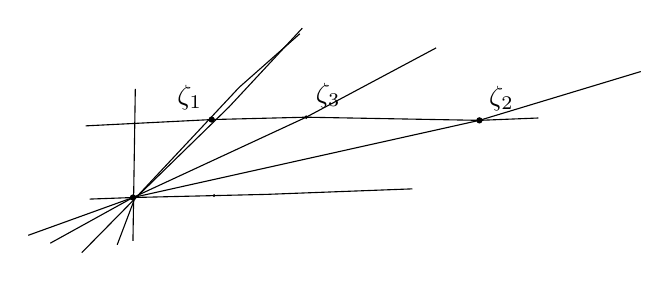
\begin{tikzpicture}[x=1cm,y=1cm]
\draw (-.65,-.7)--(.02,-.02)--(1.35,1.4)--(2.12,2.08);
\draw (-.2,-.6)--(.02,-.02)--(1.22,1.15)--(2.15,2.15);
\draw (-1.05,-.58)--(0,0)--(2.2,1.02)--(3.85,1.9);
\draw (-1.33,-.48)--(0,0)--(4.4,.98)--(6.45,1.6);
\draw (-.55,-.02)--(0,0)--(1.7,.04)--(3.55,.11);
\draw (0,-.55)--(.03,1.38);
\draw (-.6,.91)--(1,.99)--(2.2,1.02)--(4.4,.98)--(5.15,1.01);
\fill (0,0) circle(.04);
\fill (1,.99) circle(.04) node[above left] {$\zeta_1$};
\fill (2.2,1.02) circle(.025) node[above right] {$\zeta_3$};
\fill (4.4,.98) circle(.04) node[above right] {$\zeta_2$};
\fill (1.03,.025) circle(.02);
\end{tikzpicture}}

\[
\begin{array}{l}
\lambda_1\zeta_1,\lambda_1\\
\lambda_2\zeta_2,\lambda_2\\
\lambda_3\zeta_3,\lambda_3
\end{array}
\qquad
\left[\begin{gathered}
\sum\lambda_i=0\\
\sum\lambda_i\zeta_i=0\\
\text{Cela détermine }(\lambda_i)\text{ mod }\inserted{\text{mult. par}}\text{ scalaire inv.}
\end{gathered}\right.
\]
$\zeta_1,\zeta_2,\zeta_3$ tous distincts

\unsure{Or}
\[
\begin{array}{l|l}
\lambda_1=\zeta_{\underline2}-\zeta_{\underline3}&\zeta_1\\
\lambda_2=\zeta_{\underline3}-\zeta_{\underline1}&\zeta_2\\
\lambda_3=\zeta_{\underline1}-\zeta_{\underline2}&\zeta_3
\end{array}
\qquad
\left\{\begin{aligned}
\deleted{\unsure{e_2}}-e_3&=((\zeta_2-\zeta_3)\zeta_1,\zeta_2-\zeta_3)\\
\deleted{\unsure{e_3}}-e_1&=((\zeta_3-\zeta_1)\zeta_2,\zeta_3-\zeta_1)\\
\deleted{\unsure{e_1}}-e_2&=((\zeta_1-\zeta_2)\zeta_3,\zeta_1-\zeta_2)
\end{aligned}\right.
\]
\deleted{$\unsure{e_3}$}
\diagram{\begin{tikzcd}[ampersand replacement=\&]
f_1\arrow[r]\&{}
\end{tikzcd}}
\diagram{\begin{tikzcd}[ampersand replacement=\&]
(\zeta_1,1)\arrow[r,|-]\&\zeta_1f_1+
\end{tikzcd}}

\scanpage{124}
% archive foliation: 123
\begin{center}
U N I V E R S I T E\\
DES SCIENCES ET TECHNIQUES\\
DU LANGUEDOC\\
\textasciicircum\textasciicircum\textasciicircum\textasciicircum\textasciicircum\textasciicircum\textasciicircum\textasciicircum\textasciicircum\textasciicircum\textasciicircum\textasciicircum
\end{center}
Montpellier, le 4 novembre 1980

\uline{Service de la Scolarité}

AM/gs

Diffusion : Liste A\\
N° 5791

\begin{center}
\uline{AVIS DE SOUTENANCE D'UNE THESE DE DOCTEUR-INGENIEUR}

\uline{``SCIENCES DE L'EAU''}
\end{center}

\uline{NOM et prénom du candidat} : PAPPALARDO Alain

\uline{Titre de la thèse} : ``Contribution à l'étude in situ des transferts de masse dans la zone non saturée des sols''

\uline{Date, heure et lieu de soutenance prévus} : Le 12 novembre 1980 à 10 heures

Salle de cours n° 9 - Université des Sciences et Techniques du Languedoc

\uline{Nom du Directeur de thèse} : M. C. BOCQUILLON

\uline{Désignation du Laboratoire où la thèse est préparée} : Laboratoire d'Hydrologie Mathématique. U.S.T.L. Montpellier.

\uline{Analyse de l'ouvrage} : Cette étude des phénomènes dispersifs lors d'un transfert de soluté dans un milieu poreux se décompose en trois parties:

a) Mise au point du principe d'utilisation d'une sonde prototype gamma/neutrons, susceptible de détecter la présence de deutérium dans l'eau du sol. Etalonnage et test de la méthode lors d'expériences de transferts d'eau deutérée sur la colonne de laboratoire.

b) Utilisation de cette méthode non destructice d'observation en continu de la solution du sol, pour obtenir des profils de concentration, lors de 5 expériences de transfert d'eau deutérée au champ, sur sol nu, en régime hydrodynamique permanent et transitoire et sur sol cultivé couvert de luzerne, sur le site expérimental de la ferme de Cadarache (C.E.A.).

c) Essais de modélisation des résultats expérimentaux obtenus in situ. Test de plusieurs modèles numériques du transfert d'eau et de soluté : modèle monodispersif et d'hétérogénéité. Utilisation de solutions analytiques plus simples à mettre en oeuvre.

\uline{Durée approximative des recherches ayant abouti à la thèse} : 3 ans

\uline{Composition du jury proposé} :\\
MM. Cl. BOCQUILLON\\
Ph. COUCHAT\\
JP. GAUDET\\
E. SERVAT

P/ le Secrétaire Général,\\
l'Attachée d'Administration\\
Universitaire,

\uline{\unsure{Gentil}}

\uline{A. GENTIL}

\scanpage{125}
% archive foliation: 124
\[
\begin{aligned}
\zeta_1f_1+f_2&=\frac1{\zeta_2-\zeta_3}(e_2-e_3)\\
\zeta_2f_1+f_2&=\frac1{\zeta_3-\zeta_1}(e_3-e_1)\\
\zeta_3f_1\unsure{+}f_2&=\frac1{\zeta_1-\zeta_2}(e_1-e_2)
\end{aligned}
\]
\diagram{\begin{tikzcd}[ampersand replacement=\&,column sep=0pt,row sep=large]
(\zeta_1-\zeta_2)f_1=\frac1{\zeta_3-\zeta_1}e_1+\frac1{\zeta_2-\zeta_3}e_2\unsure{-}
\&
\left(\underbrace{\frac1{\zeta_3-\zeta_1}+\frac1{\zeta_2-\zeta_3}}\right)e_3
\arrow[d,bend left=35]\\
f_1=\frac1{(\zeta_1-\zeta_2)(\zeta_3-\zeta_1)}e_1+
\frac1{(\zeta_1-\zeta_2)(\zeta_2-\zeta_3)}e_2-
\&
\frac1{(\zeta_1-\zeta_2)}(\phantom{xx})e_3
\end{tikzcd}}
\[
\begin{aligned}
f_2&=\frac1{\zeta_2-\zeta_3}(e_2-e_3)-\zeta_1f_1\\
&=-\frac{\zeta_1}{(\zeta_1-\zeta_2)(\zeta_3-\zeta_1)}e_1+
\left(\frac1{\zeta_2-\zeta_3}-\frac{\zeta_1}{(\zeta_1-\zeta_2)(\zeta_2-\zeta_3)}\right)e_2\\
&\qquad+\left[-\frac1{\zeta_2-\zeta_3}
+\frac{\zeta_1}{\zeta_1-\zeta_2}
\left(\frac1{\zeta_3-\zeta_1}+\frac1{\zeta_2-\zeta_3}\right)\right]e_3
\end{aligned}
\]
\[
\begin{aligned}
(\zeta_1-\zeta_2)(\zeta_2-\zeta_3)(\zeta_3-\zeta_1)f_2
={}&-\zeta_1(\zeta_2-\zeta_3)e_1+
\left[\underbrace{\underbrace{(\zeta_1-\zeta_2)(\zeta_3-\zeta_1)}}\right.\\
&\left.\quad\unsure{-}\zeta_1(\zeta_3-\zeta_1)\right]e_2+
\left[\unsure{-}(\zeta_1-\zeta_2)(\zeta_3-\zeta_1)\right.\\
&\left.\quad+\zeta_1(\zeta_2-\zeta_3)+\zeta_1(\zeta_3-\zeta_1)\right]e_3
\end{aligned}
\]
\figure{\begin{tikzpicture}[x=1cm,y=1cm]
\draw (0,0)--(.12,.27);
\draw (2.15,0)--(2.3,.3);
\end{tikzpicture}}
\[
-\zeta_1(\zeta_2-\zeta_3)e_1
\unsure{-}\zeta_2(\zeta_3-\zeta_1)e_2
-\zeta_3(\zeta_1-\zeta_2)e_3
\]

\scanpage{126}
% archive foliation: 125
\[
\deleted{\zeta_1(\zeta_2-\zeta_3)\qquad\zeta_2(\zeta_3-\zeta_1)}
\]
\[
(\zeta_1-\zeta_2)(\zeta_2-\zeta_3)(\zeta_3-\zeta_1)=\Delta_0
\]
\[
\boxed{\begin{aligned}
-\Delta_0f_2&=\zeta_1(\zeta_2-\zeta_3)e_1\unsure{+}\zeta_2(\zeta_3-\zeta_1)e_2+\zeta_3(\zeta_1-\zeta_2)e_3\\
\unsure{\cdot|-}\Delta_0f_1&=(\zeta_2-\zeta_3)e_1+(\zeta_3-\zeta_1)e_2+(\zeta_1-\zeta_2)e_3
\end{aligned}}
\]
$t$ correspond donc à
\[
\begin{aligned}
&\sum(\zeta_j-\zeta_k)e_i\\
={}&\sum_i(\wp(\varepsilon_j)-\wp(\varepsilon_k))e_i
\end{aligned}
\]

\scanpage{127}
% archive foliation: 126
\begin{center}
UNIVERSITE DES SCIENCES ET TECHNIQUES\\
DU LANGUEDOC\\
Institut de Mathématiques\\
Place Eugène Bataillon\\
34060 MONTPELLIER CEDEX
\end{center}

Dans le cadre des conférences d'intérêt général, Monsieur JAMBON parlera le Vendredi 12 décembre 1980, à 14h30, Salle de cours n° 4 sur le sujet suivant :

\begin{center}
LES NOMBRES ENTIERS :

UNE PRESENTATION EN TERMES DE LANGAGE ALGORITHMIQUE
\end{center}

Vous êtes invité à cette conférence et au thé des mathématiciens qui suivra à 16 h dans la Salle de Réunion du Bâtiment de Mathématiques.

M. LEFRANC\\
Directeur de l'U.F.R. 5

\scanpage{128}
% archive foliation: 127
Relations entre $M_{11}$\\
et $M_{04}$

\scanpage{129}
% archive foliation: 128
Approche transcendante
% Pencilled page-count annotation; hand not securely attributed.
\margin{(\unsure{22|21} p)}

\scanpage{131}
% archive foliation: 130
Modules des courbes elliptiques : théorie transcendante

La donnée d'une courbe elliptique \inserted{$E$} sur $\mathbb C$ revient à celle \deleted{à} d'un \inserted{$\mathbb C$} espace vectoriel de rang $1$, savoir $t_E$
\[
\tag{1}
V=t_E\qquad\text{(espace tangent à l'origine)}
\]
et d'un ``réseau''
\[
\tag{2}
H\subset V
\]
(un \deleted{groupe abélien} \inserted{$\mathbb Z$-module} \deleted{discret} \inserted{discret, libre} de rang $2$). La donnée du \deleted{groupe} $\mathbb Z$-module $\unsure{\Pi|H}$ permet de récupérer $V$ en tant qu'espace vectoriel réel \inserted{(de rang $2$)} par
\[
\tag{3}
V\simeq H\otimes_{\mathbb Z}\mathbb R\overset{\text{déf}}=H_{\mathbb R}
\]
et $E$ en tant que groupe de Lie réel, par
\[
\tag{4}
E\simeq V/H\simeq H_{\mathbb R}/H,
\]
tandis que la structure complexe de $E$ est déterminée par la donnée d'une structure d'espace vectoriel complexe sur $V$ par passage aux quotients.

Étant donné un espace vectoriel réel $V$, \inserted{\deleted{de rang $2$}} la donnée d'une structure complexe sur $V$ (i.e. d'un endom $u$ de $V$ de carré $-\mathrm{id}_V$) équivaut aussi à celle d'un \inserted{$\mathbb C$-}sous-espace vectoriel $L$ de $V_{\mathbb C}$
\[
\tag{5}
V_{\mathbb C}=V\otimes_{\mathbb R}\mathbb C
\]
tel que la projection canonique
\[
\tag{6}
\begin{aligned}
V_{\mathbb C}&\longrightarrow V=V_{\mathbb R}\\
z&\longmapsto\tfrac12(z+\bar z)=\Re z
\end{aligned}
\]
\deleted{soit} \inserted{induit} un isomorphisme d'espaces vectoriels réels.
\[
\tag{7}
\deleted{\text{Pour un}}\quad\varphi:L\xrightarrow{\sim}V\quad(\mathbb R\text{-iso})
\]

\scanpage{132}
% archive foliation: 131
À un tel $L$, on associe la structure complexe
\inserted{\deleted{\unsure{conjuguée}} \deleted{\unsure{directe}}, \deleted{conjuguée de celle déduite de}}
\deleted{$V$ \unsure{directe} de celle de $L$ par transport de}
$V$ qui est conjuguée de celle déduite de la str. complexe de $L$ par transport de structure via (7), i.e. on pose
\[
\tag{8}
ux=\varphi(-i\varphi^{-1}(x))=-\varphi(i\varphi(x))
\]
\margin{$u$ étant la multiplication par $i$ pour la structure complexe envisagée sur $V$}
\margin{cette convention est imposée par les \unsure{structures} de ``\unsure{modules}'' de courbes elliptiques \unsure{et de VA)}, du fait qu'on veut que les param. modulaires \unsure{qu'on} \unsure{(*)} introduit soient \uline{holomorphes} et non antiholomorphes \ldots}

Inversement, si $V$ est muni d'une structure complexe, \deleted{l'applic} faisant de $V$ un espace vectoriel complexe $V_c$, alors l'application \inserted{identique} $\mathbb R$-linéaire $V\longrightarrow V_c$ se prolonge, par la propriété universelle de $V_{\mathbb C}$, en une application $\mathbb C$-linéaire
\[
\tag{9}
\psi:V_{\mathbb C}\longrightarrow V_c
\]
de sorte que
\[
\tag{10}
\left\{\begin{aligned}
\psi(ix)&=ux\\
\psi(x)&=x
\end{aligned}\right.
\qquad\forall x\in V=V_{\mathbb R},
\]
donc
\[
\tag{11}
\psi(x+iy)=x+uy.
\]
\deleted{Posons} \deleted{Considérons} Considérons
\[
\tag{12}
\begin{aligned}
L^{\unsure{\prime|!}}=\operatorname{Ker}\psi
&=\{x+iy\mid x,y\in V_{\mathbb R},\ x+uy=0\ \text{i.e. }y=\unsure{u}x\}\\
&=\{\deleted{\unsure{x+iu(x)}}\mid x\in V_{\mathbb R}\}
\end{aligned}
\]
et considérons l'application correspondante (6)
\[
\begin{gathered}
\varphi:\underset{\substack{\Vert\\x+iu(x)}}z\longmapsto\tfrac12(z+\bar z)
=\Re z=x\deleted{\unsure{+uy}}:\quad L\longrightarrow V .
\end{gathered}
\]
On voit alors que cette application est bijective, et \uuline{antilinéaire},
\inserted{et que la \unsure{correspondance} à la structure complexe}
\deleted{\unsure{permet de récupérer la structure complexe primitive sur $V_{\mathbb R}$}},
\deleted{$L=L^{\unsure{\prime|!}}=\operatorname{Ker}\psi\ \unsure{\subset V_{\mathbb C},\ V=L_{\mathbb R}}$},
\margin{\unsure{voir une autre explication}}

(13) $[$On peut dire aussi, que la donnée d'une structure complexe sur $V$ équivaut :

1°) La donnée d'un \deleted{\unsure{gr}} sous-groupe compact \deleted{maximal} $U$ \deleted{de} \deleted{$\unsure{\mathrm{Gl}}$} $\in\operatorname{Aut}_{\mathbb R}(V)$, \deleted{i.e. d'un}

\scanpage{133}
% archive foliation: 132
\deleted{\unsure{de sous-groupe}} isomorphe à $\mathbb U=\{z\in\mathbb C\mid |z|=1\}$, \inserted{tel que l'action sur $V_{\mathbb C}$ ait exactement $2$ sous-espaces propres}
\margin{(c'est automatique si $\operatorname{rg}_{\mathbb R}V=2$)}

$2^\circ)$ D'un des deux éléments d'ordre $4$ de $U$, ou ce qui revient au $=$, d'une \uline{orientation} de $U$, ou encore \inserted{(si $\operatorname{rg}_{\mathbb R}V=2$, plus gén. si $\operatorname{rg}_{\mathbb R}V=2n$, $n$ impair)} d'une orientation de $V$.
\margin{ou encore d'un \inserted{des deux} isomorphismes $\mathbb U\xrightarrow{\sim}U$, $U\xrightarrow{\sim}\mathbb U$}

--- l'élément d'ordre $4$ de $U$ associé à une orientation $\omega$ de \inserted{$U$ (ou de} $V$\inserted{)} sera noté $u_\omega$, c'est donc la rotation de $+\pi/2$ pour l'orientation \inserted{$\omega$} de $V$ et toute structure \deleted{\unsure{euclidienne}}\inserted{euclidienne} sur $V$ choisie invariante sous $U$ (\uline{NB} \inserted{si $\operatorname{rg}_{\mathbb R}V=2$,} une telle \deleted{\unsure{structure}}\inserted{métrique} est unique à scalaire multiplicatif près).

Alors $V_{\mathbb C}$ sous l'action de $U$ se décompose en deux sous-espaces propres
\begin{equation}
V_{\mathbb C}=\bigoplus_{\omega\in\underline\omega}L_\omega
\tag{\unsure{14|16}}
\end{equation}
où pour $\omega\in\underline\omega(U)=\underline\omega$, $L_\omega$ est caractérisé par le fait que l'isomorphisme
\begin{equation}
\varphi_\omega:U\xrightarrow{\sim}\mathbb U
\qquad
g(z)=\varphi_\omega(g)\cdot z\quad\text{pour }z\in L_\omega
\tag{15}
\end{equation}
défini par l'action de $U$ sur $L_\omega$, \unsure{corresponde|correspond} à l'orientation $\omega$. La donnée d'une structure complexe sur $V$ \inserted{compatible avec $U$} équivaut alors à celle d'un des deux isomorphismes $\varphi_\omega$ (permettant de faire opérer $\mathbb U$ sur $V$, donc aussi $\mathbb R^{\times+}\times\mathbb U\simeq\mathbb C^\times$, \deleted{\unsure{donc}} $\mathbb C\ldots$). Ceci dit, pour $\deleted{\unsure{z\in\mathbb C}}\ z\in L_\omega$, on aura
\[
\operatorname{Re}(\varphi_\omega(g)z)=\operatorname{Re}(gz)=g\operatorname{Re}(z)
=\text{produit de }\operatorname{Re}(z)\text{ par }\varphi_\omega(g)
\text{ pour la structure complexe de }V\text{ associée à }\varphi_\omega.
\]

\scanpage{134}
% archive foliation: 133
i.e.
\figure{\begin{tikzpicture}\draw (0,0)--(0,.32);\end{tikzpicture}}
\diagram{\begin{tikzcd}[ampersand replacement=\&]
L_\omega \arrow[r, no head, "\sim"] \& V\\
z \arrow[r, mapsto] \& \operatorname{Re}z
\end{tikzcd}}
est un isomorphisme d'espaces vectoriels complexes, quand on munit $V$ de la structure complexe $c_\omega$. ]

\margin{Mais il y a lieu d'associer à cette structure complexe sur $V$ \unsure{non pas} $L_\omega$, mais $L_{\omega'}$, cf. plus bas\ldots}

Dans le cas qui nous occupe, $\operatorname{rg}_{\mathbb R}V=2$ les \deleted{droites} sous-espaces vectoriels envisagés de $V_{\mathbb C}$ sont de \deleted{$\unsure{\operatorname{rg}}$} $\operatorname{rg}1$, \inserted{$\operatorname{corg}1$,} et peuvent s'interpréter comme les points de
\begin{equation}
\Sigma=\Sigma_V=P(\mathbb C),\quad\text{où }P=\mathbb P(V)
\tag{16}
\end{equation}
est le \deleted{\unsure{esp.}} schéma droite projective réelle associé à $V$. Pour que
\diagram{\begin{tikzcd}[ampersand replacement=\&]
L \arrow[r] \& V\\
z \arrow[r, mapsto] \& \operatorname{Re}z
\end{tikzcd}}
soit un isomorphisme, i.e. pour que $L$ corresponde à une structure complexe \deleted{de} sur $V$, il faut que \deleted{le point $z$ correspondant de $\Sigma$ ait \unsure{une pensée|une partie}} \inserted{$L\cap V=\{0\}$ i.e. $L$} n'est pas complexifié d'une droite $L_0\subset V_{\unsure{\mathbb R}}$; i.e. que le point $z\in\Sigma$ qui correspond à $L$ \inserted{ne} soit pas dans $\deleted{\Sigma(\mathbb R)}$
\[
\Sigma_{\mathbb R}=P(\mathbb R)
\]
ou encore qu'on ait
\begin{equation}
z\in\Sigma\setminus\Sigma_{\mathbb R}.
\tag{17}
\end{equation}
\deleted{\unsure{En résumé}} Ainsi, les structures complexes

\scanpage{135}
% archive foliation: 134
sur $V$ sont en correspondance biunivoque avec l'ens $\Sigma\setminus\Sigma_{\mathbb R}$ des points non réels de $\Sigma$.

Notons que l'ens $\Sigma\setminus\Sigma_{\mathbb R}$ a deux composantes connexes \inserted{$\Sigma_\omega^*$}, qui correspondent (par Stokes) aux deux orientations de $\Sigma_{\mathbb R}$, ou encore aux deux orientations de $V$.

La composante connexe d'un $z\in\Sigma\setminus\Sigma_{\mathbb R}$ correspond à l'orientation de $V$ définie de façon évidente par la structure complexe envisagée sur $V$ (définie par $z$).
\margin{C'est faux, cf calcul plus bas}

Revenant à la description transcendante des courbes elliptiques, on voit qu'\inserted{la donnée d'}une telle courbe $E$ revient à la donnée

a) D'un $\mathbb Z$-module libre de rang $2$ $H$

b) D'une \deleted{droite} orientation $\omega$ de $V=\unsure{\Pi|H}\otimes_{\mathbb Z}\mathbb R$, ou ce qui revient au $=$, d'une des deux bases de $\bigwedge_{\mathbb Z}^{2}H$ (i.e. d'une restriction du groupe structural $\mathrm{Gl}(2,\mathbb Z)$ de $H$ à $\mathrm{Sl}(2,\mathbb Z)$), \inserted{\deleted{soit} notée aussi $\omega$}
\margin{On a $H=\pi_1(E,0_E)$\\
$V=H\otimes_{\mathbb Z}\mathbb R\simeq t_E$}

c) D'un point $z\in\Sigma_\omega(V)$,

Une \uline{rigidification de Torelli} de la courbe elliptique $E$ est la donnée d'un isomorphisme

\scanpage{136}
% archive foliation: 135
\begin{equation}
\mathbb Z^2\longrightarrow H
\tag{18}
\end{equation}
compatible avec les orientations, i.e. tel que l'on ait
\begin{equation}
z_1\wedge z_2=\omega
\tag{19}
\end{equation}
où $z_1,z_2$ sont les images par (18) des éléments de la base canonique de $\mathbb Z^2$. Cet isomorphisme (18) définit un isomorphisme correspondant
\begin{equation}
\mathbb R^2\simeq V
\tag{20}
\end{equation}
d'où des isomorphismes
\begin{equation}
\left\{
\begin{aligned}
\mathbb P_{\mathbb R}^1&\simeq\mathbb P^1(V),&
\mathbb P^1(\mathbb C)&\simeq\Sigma_V\\
\mathcal D&\simeq\Sigma_{V,\omega}^*
\end{aligned}
\right.
\tag{21}
\end{equation}
où $\mathcal D$ est le demi-plan de Poincaré, i.e. \deleted{l'ens} la variété complexe des $z\in\mathbb C$ tels que $\deleted{\unsure{\Im z}}\ \Im z>0$
\begin{equation}
\mathcal D=\{z\in\mathbb C\mid\Im z>0\},
\tag{22}
\end{equation}
identifié à $\Sigma_{\mathbb R^2,\omega_0}^*$ en identifiant $z\in\mathcal D$ à la droite
\begin{equation}
L_z\deleted{\unsure{R_z}}=\mathbb C\cdot\underbrace{(z,1)}_{ze_1+e_2}.
\tag{23}
\end{equation}

\margin{$(e_1,e_2)$ base canonique de $\mathbb R^2$. Si on associait à $z\in\mathbb C$ la droite $\mathbb C(1,z)$, alors $\Sigma_{\mathbb R^2,\omega_0}^*$ correspondrait au demi-plan $\mathcal D^-$ au lieu de $\mathcal D=\mathcal D^+$.}

\margin{Ainsi, les classes d'isomorphie de courbes elliptiques avec rigidif. de Torelli sont en corr. biuniv. \unsure{avec l'ens} des pts de $\mathcal D$.}

Sur l'ens des classes d'isomorphie de courbes elliptiques $E=(\unsure{\Pi|H},\omega,L\subset H\otimes_{\mathbb Z}\mathbb C)$, avec rigidification de Torelli $\mathbb Z^2\simeq H$, le groupe $\mathrm{Sl}(2,\mathbb Z)$ opère à droite de façon évidente, par composition \inserted{à droite} de (18) avec les automorphismes de $\mathbb Z^2$. \deleted{\unsure{Comme on}}

\scanpage{137}
% archive foliation: 136
expliciter cette action en tant qu'action sur $\mathcal D$ (défini par (22)).

Si une structure complexe sur $\mathbb R^2$ est définie par l'élément $z\in\mathcal D$, $z=\unsure{x}+iy$, alors l'application \inserted{$\unsure{\mathbb R|\mathbb C}$-linéaire} $\varphi:L_z=\mathbb C(z,1)\longrightarrow V$ s'identifie à:
\[
\underset{\substack{\Vert\\a+ib}}{\lambda}\longmapsto
\operatorname{Re}\bigl(\deleted{\unsure{x}}\underbrace{\lambda(ze_1+e_2)}_{[(ax-by)+i(ay+bx)]e_1+(a+ib)e_2}\bigr)
=(ax-by)e_1+ae_2
\]
les images inverses $\lambda_1,\lambda_2$ de $e_1,e_2$ dans celle-ci sont données par
\[
\lambda_1=-\frac{i}{y}\qquad
\lambda_2=1+i\frac{x}{y}
\]
d'où
\[
\lambda_2/\lambda_1=i(y+ix)=-x+iy
\]
donc on a
\[
\underbrace{e_2/e_1}_{\substack{\text{quotient dans }\mathbb C^*\\
\text{au sens de la}\\
\text{structure compl. de }\mathbb R^2\\
\text{définie par }z=x+iy\in\mathcal D}}
=\overline{(-x+iy)}=-x-iy=-z
\quad\in\mathcal D^-.
\]

Donc si une structure de Torelli sur $E$ est définie par la \deleted{\unsure{donnée}}\inserted{base} $(z_1,z_2)$ de $\Pi\subset t_E$, alors l'élément $z\in\mathcal D$ correspondant est donné par
\begin{equation}
\deleted{z_2/z_1=-x+iy=-\overline z\quad\text{où }z=x+iy.}
\qquad\inserted{z=-(z_2/z_1)}
\tag{24}
\end{equation}

Soit donc
\[
g\in\mathrm{Sl}(2,\mathbb Z)\qquad
g=\begin{pmatrix}a&b\\c&d\end{pmatrix}
\qquad
\begin{gathered}
a,b,c,d\in\mathbb Z\\
ad-bc=1
\end{gathered}
\]
et soit \deleted{\unsure{un u}} $u:\mathbb Z^2\xrightarrow{\sim}\Pi$ une structure de Torelli, correspondant à

\scanpage{138}
% archive foliation: 137
\[
z_1=u(e_1),\ z_2=u(e_2)\in H\subset V
\]
alors la structure de Torelli $\uline{u\circ g}$ correspond à $z'_1,z'_2\in\Pi$ donnés par
\[
\begin{aligned}
z'_1&=ug(e_1)=u(ae_1+ce_2)=az_1+cz_2\\
z'_2&=ug(e_2)=u(be_1+de_2)=bz_1+dz_2,
\end{aligned}
\]
qui correspond donc à un élément
\[
z'=x'+iy'\in\mathcal D'
\]
donné par
\deleted{\unsure{(24)}}
\begin{equation}
z'\deleted{\unsure{(x'+iy')}}=
-\frac{z'_2}{z'_1}
=-\frac{bz_1+dz_2}{az_1+cz_2}
=-\frac{d\frac{z_2}{z_1}+b}{c\frac{z_2}{z_1}+a}
=\frac{d\unsure{z|\overline z}\unsure{-|+}b}{-c\unsure{z|\overline z}+a}
\tag{25}
\end{equation}
\deleted{$\unsure{\widetilde z'=-\overline{z'}}$}

où $\deleted{\unsure{\widetilde z=x+iy=-\overline z}}$.
\margin{\diagram{\begin{tikzcd}[ampersand replacement=\&,column sep=small,row sep=large]
 \& z'=\unsure{\frac{-dz+b}{-cz+a}} \arrow[dl,bend right=55] \arrow[d,bend left=50] \arrow[d,bend right=25] \\
\unsure{(?)} \& z'=\unsure{\frac{dz-b}{-cz+a}} \arrow[l,bend left=35] \arrow[u,bend left=35]
\end{tikzcd}}}

Si on \deleted{\unsure{veut}} préfère expliciter l'action à gauche $u\longmapsto u\circ g^{-1}$ de $\mathrm{Sl}(2,\mathbb Z)$ sur l'ens. des structures de Torelli mod iso, on voit que
\[
g^{-1}=\begin{pmatrix}d&-b\\-c&a\end{pmatrix}
\qquad\deleted{\text{d'où}}
\]
d'où maintenant, pour $z'=x'+iy'$ correspondant à $u\circ g^{-1}$
\deleted{\unsure{(25 bis)}}
\[
\deleted{\widetilde z'=\overline{z'}
=\frac{a\widetilde z-b}{-c\widetilde z+d}
=\frac{-a\overline z-b}{-c\overline z-d}
=\unsure{\frac{a\overline z+b}{c\overline z+d}|\overline{\frac{az+b}{cz+d}}}}
\]
\begin{equation}
z'=\frac{az+b}{cz+d}
\tag{25 bis}
\end{equation}
\uline{victoire}, c'est la formule habituelle,

mais on fera attention que le nb complexe $z\in\mathcal D$ attaché à la structure de Torelli définie par \deleted{$z_1,z_2\in t_E$}\inserted{les deux} éléments $z_1,z_2$ de la droite complexe $\deleted{\unsure{t=\lambda}}\ t_E$ est donné, non

\scanpage{139}
% archive foliation: 138
\deleted{par la formule $z_2/z_1$, qu'on} pourrait penser $z=z_2/z_1$, \deleted{\unsure{et}} mais par $(24\deleted{\unsure{bis}})$ i.e. par
\[
z=-\unsure{\overline{(z_2/z_1)}|(z_2/z_1)^{-1}}
=-\unsure{\overline{z_2}/\overline{z_1}|z_2/z_1}\in\mathcal D.
\]
Si on voulait repérer \inserted{non} la structure de Torelli par le nb $z\in\mathcal D$ choisi, mais par le nb complexe $\tau=z_2/z_1$ lui-même (symétrique de $z$ p.r. à l'axe imaginaire), on trouverait une formule de transformation d'opération de $\mathrm{Sl}(2,\mathbb Z)$ sur $\mathcal D$ qui n'est \uline{pas} la formule habituelle.

\margin{Donc cela montre que la condition $z\in\mathcal D^+$ signifie que $(z_1,z_2)$ est, non une base directe, mais une base \uline{inverse} de $\unsure{t_E}$. Si on \deleted{voulait}\inserted{veut} faire correspondre à $z\in\mathcal D^+$ une structure de Torelli (directe), il y a lieu de changer la convention (23) en $L_z=\mathbb C(1,z)$ qui donne une \deleted{\unsure{orientation}}\inserted{structure complexe sur $\mathbb R^2$} compatible avec l'orientation canonique (car $L_z\in\Sigma_{\mathbb R^2,\omega_0}^{-}$, cf \unsure{calcul ci-dessus}). On trouve
\[
\uline{z=-(z_2/z_1)^{-1}=-\frac{z_1}{z_2}}.
\]
C'est un point \unsure{auquel il|où il} faudrait vérifier que le foncteur en question est bien analytiquement naturel\ldots}

On trouve ici le

\uline{Théorème} $\mathcal D$ \inserted{$=\{z\in\mathbb C\mid\Im z>0\}$,} muni de la famille \inserted{analytique} de courbes elliptiques
\[
E_z=\mathbb C/(\mathbb Z\cdot1+\mathbb Z\cdot(-\overline z))
\]
est un revêtement universel de $M_{1,1}^{\mathrm{an}}$, correspondant à la classification des courbes elliptiques avec rigidification de Torelli; le groupe des $M_{1,1}^{\mathrm{an}}$-automorphismes de $\mathcal D$ (opérant à droite) s'identifie au groupe $\mathrm{Sl}(2,\mathbb Z)$, opérant sur $\mathcal D$ par
\[
gz=\frac{az+b}{cz+d}\qquad\text{pour }\quad
g=\begin{pmatrix}a&b\\c&d\end{pmatrix}\in\mathrm{Sl}(2,\mathbb Z),
\]
qui correspond ainsi à l'opération à g. naturelle

\scanpage{140}
% archive foliation: 139
de $\unsure{\mathrm{Gl}|\mathrm{Sl}}(2,\mathbb Z)$ sur les structures de Torelli, par
\[
g\cdot u=u\circ g^{-1}\qquad
(u:\mathbb Z^2\xrightarrow{\sim}\pi_E).
\]

\uline{Corollaire 1} On a un iso. canonique
\begin{equation}
\mathcal T_{1,1}\simeq\mathrm{Sl}(2,\mathbb Z)
\tag{26}
\end{equation}
(où $\mathcal T_{11}=\pi_1(M_{1,1})$ est calculé relativement au revêtement universel choisi $\mathcal D$ de $M_{1,1}$).
\inserted{On a un iso. can
\begin{equation}
M_{1,1}\simeq(\unsure{\mathcal D},\mathrm{Sl}(2,\mathbb Z))
\tag{27}
\end{equation}}

Utilisant les grands théorèmes \unsure{marteaux-pilons}, on en déduit

\uline{Corollaire 2} Soit \deleted{$(E,a)$} une surface orientée \inserted{ponctuée} compacte connexe de genre $1$, et soit $\mathcal T$ le groupe des classes d'isotopie des automorphismes de $(E,a)$. \deleted{Alors considérons}\inserted{Alors} l'homomorphisme naturel
\begin{equation}
\mathcal T\longrightarrow\operatorname{Aut}_{\mathbb Z}^{+}(H)
\qquad\text{où }\quad H=\pi_1(E,a)
\tag{27}
\end{equation}
est un isomorphisme. $\unsure{\S}$

\uline{Corollaire 3} Soit $\Pi$ un groupe à lacets du type $\unsure{g}(1,1)$, $H=\Pi_{\mathrm{ab}}$ (qui est un $\mathbb Z$-module libre de rang $1$), $\mathcal T=\operatorname{Autext}^{+}_{\mathrm{lac}}(\Pi)$, \deleted{considérons}\inserted{alors, l'hom}
\begin{equation}
\mathcal T\longrightarrow\operatorname{Aut}_{\mathbb Z}^{+}(H)
\tag{28}
\end{equation}
est iso.

\margin{Il faudrait expliciter l'action \unsure{extérieure} de $\operatorname{Aut}_{\mathbb Z}^{+}(H)$ sur $\Pi$ via \unsure{l'action|l'identif.} $\operatorname{Aut}_{\mathbb Z}^{+}(H)\ldots$}

\scanpage{141}
% archive foliation: 140
\margin{$\deleted{\unsure{P_{\mathcal D}}}$}

Nous pouvons expliciter le fibré tangent le long \unsure{de|des} \deleted{fibres}\inserted{la section nulle} de la courbe elliptique universelle rigidifiée à la Torelli, comme étant le fibré formé des $t_E$, qui du point de vue fibré vectoriel réel s'identifie au \deleted{fibré} $\mathrm{Sl}(2,\mathbb Z)$-fibré sur $\mathcal D$ défini par l'opération \unsure{standart|standard} de $\mathrm{Sl}(2,\mathbb Z)$ sur $\mathbb R^2$. Le fibré principal associé \inserted{$P_{\mathcal D}$} s'obtient donc (pour sa seule structure topologique) en remplaçant dans cet énoncé $\mathbb R^2$ par $(\mathbb R^2)^*$.

Pour en trouver un revêtement universel, il suffit de choisir un revêtement universel de $(\mathbb R^2)^*\simeq\mathbb C^*$, p.ex. le revêtement par l'exponentielle complexe
\[
z\longmapsto\exp(2i\pi z):\quad
\mathbb C\longrightarrow\mathbb C^*.
\]

\scanpage{143}
% archive foliation: 142
$\cdot$ Une courbe elliptique $E$ sur $\mathbb C$ est déterminée par
\begin{equation}
\left\{
\begin{array}{l}
\text{a) ``réseau'' }H,\ \deleted{\unsure{\phi}}\ \mathbb Z\text{-module libre de rang }2
\qquad\deleted{\unsure{(H=1}}\\
(H=\pi_1(E,0_E)\simeq H_1(E,\mathbb Z)\simeq H^1(E,\mathbb Z)^\vee)\\
\text{b) Une structure complexe sur }V=H\otimes_{\mathbb Z}\mathbb R\ \deleted{\unsure{\simeq V}}\
(\simeq t_E,\\
\qquad\text{espace tangent à l'origine de }E).
\end{array}
\right.
\tag{1}
\end{equation}

La donnée a) permet de reconstituer $E$ comme groupe de Lie réel par
\begin{equation}
E\simeq H\otimes_{\mathbb Z}\mathbb R/H
\tag{2}
\end{equation}
et la donnée b) redonne la structure complexe sur $E$, par passage au quotient.

Quand on est sur une base $S$, espace $\mathbb C$-analytique, la donnée a) correspond à un système local $\mathcal H$ sur $S$ --- faisceau en $\mathbb Z$-modules loc libres de rang $2$ sur $S$, d'où un fibré vectoriel $\mathbb R$-analytique $\mathcal H\otimes_{\mathbb Z}\mathbb R$ sur $S$. La structure b) correspond à une structure complexe \deleted{sur} de ce dernier, en tant que fibré vectoriel \inserted{complexe} de rang $1$, de façon que les sections locales de $\mathcal H$ deviennent des sections analytiques complexes. Si \deleted{$\unsure{e}$} $z_1,z_2$ sont deux sections de $\mathcal H$ formant

\scanpage{144}
% archive foliation: 143
une base de $\mathcal H\otimes_{\mathbb Z}\mathbb R$ (\inserted{fibre par fibre} sur $\mathbb R$), la donnée d'une telle structure complexe équivaut à la donnée de
\begin{equation}
\tau=z_2/z_1
\tag{3}
\end{equation}
en tant que section du faisceau structural $\mathcal O_S$. (\uline{NB} \deleted{il faut,} Pour une structure complexe donnée sur $\mathcal H\otimes_{\mathbb Z}\mathbb R$, $z_1$ et $z_2$ sont deux sections\inserted{-bases} du faisceau inversible obtenu, et $\tau$ est la section de $\underline{\mathcal O}_S$ qui fait passer de l'une à l'autre:
\begin{equation}
z_2=\tau z_1.
\tag{3 bis}
\end{equation}
\margin{Noter que $\forall s$, $\tau(s)\in\mathbb C\setminus\mathbb R$}

Une structure \uline{de Torelli} sur une \deleted{\unsure{fam}} courbe elliptique relative $E$ sur $S$ (correspondant à: $\mathcal H$ sur $S$ $+$ structure complexe sur $\mathcal H\otimes_{\mathbb Z}\mathbb R$) est la donnée d'un isomorphisme
\begin{equation}
t:\mathbb Z_S^2\xrightarrow{\sim}\mathcal H,
\tag{4}
\end{equation}
\deleted{\unsure{ou d'}}\inserted{ou encore} \deleted{une} de deux sections $z_1,z_2$ de $\mathcal H$, \deleted{\unsure{satisfais}} formant une base de $\mathcal H$ en tte fibre. La catégorie des courbes elliptiques relatives, sur $S$, avec structure de Torelli, \unsure{c'est|est} \deleted{équivalente à}\inserted{``rigide''}\deleted{est} (pas d'autom. $\ne\mathrm{id}$ d'un objet) et l'ens des

\scanpage{145}
% archive foliation: 144
classes d'isomorphie d'objets d'icelle est en corr. biunivoque canonique avec l'ens des applications holomorphes
\begin{equation}
\tau:S\longrightarrow\mathbb C\setminus\mathbb R.
\tag{5}
\end{equation}
On dit qu'une structure de Torelli est ``directe'' ou ``stricte'' si \deleted{$t$ est} pour tt $s\in S$, la base \deleted{de} $z_1,z_2$ de $\mathcal H_s\otimes_{\mathbb Z}\mathbb R$ \deleted{correspond à}\inserted{définit} l'\deleted{\unsure{structure}}orientation de cet espace correspondant à sa structure complexe, i.e. si (5) est un morphisme
\begin{equation}
\tau:S\longrightarrow\mathcal D^+=\{z\in\mathbb C\mid\Im z>0\}.
\tag{6}
\end{equation}
Donc $\mathcal D^+$ apparaît comme l'espace analytique modulaire pour la structure ``courbe elliptique relative avec str. de Torelli stricte sur espace analytique variable'', la famille modulaire étant donnée par
\begin{equation}
\unsure{\mathcal X|\mathfrak X}_{\mathcal D^+}=(\mathcal D^+\times\mathbb C)/\mathbb Z^2
\tag{7}
\end{equation}
où $\mathbb Z^2$ opère sur $\mathcal D^+\times\mathbb C$ par
\begin{equation}
\deleted{\unsure{u}}\ T_{m,n}(\tau,z)=(\tau,z+m+n\tau)
\qquad\tau\in\mathcal D^+,\ z\in\mathbb C
\tag{8}
\end{equation}
de sorte que l'on a
\begin{equation}
(\unsure{\mathcal X|\mathfrak X}_{\mathcal D^+})_\tau
\simeq\mathbb C/(\mathbb Z+\mathbb Z\cdot\tau)
\simeq\mathbb C^*/\substack{\text{sous-groupe}\\
\text{engendré}\\
\text{par }\deleted{\unsure{q}}\ \unsure{\kappa|k}=\exp(2i\pi\tau)\\
(\text{satisfaisant }|\unsure{\kappa|k}|<1)}
\tag{8}
\end{equation}

\scanpage{146}
% archive foliation: 145
Sur l'ens des \deleted{structures} classes d'isomorphie de structures de Torelli directes, le groupe
$\deleted{\unsure{\mathrm{Sl}(2)}}$
\begin{equation}
\mathrm{Sl}(2,\mathbb Z)=
\left\{\begin{pmatrix}a&b\\c&d\end{pmatrix}
\ \middle|\ 
\begin{gathered}
a,b,c,d\in\mathbb Z\\
ad-bc=1
\end{gathered}\right\}
\tag{9}
\end{equation}
opère à droite, par
\[
t\mathrel{\unsure{\mapstochar\relbar\relbar|\longmapsto}}t\circ g,
\]
on va expliciter cette opération, en tant qu'opération sur $\mathcal D^+$, et $=$ sur $\unsure{\mathcal X|\mathfrak X}_{\mathcal D^+}$ (vu que l'on a une opération de $\mathrm{Sl}(2,\mathbb Z)$ sur la situation modulaire).

On voit qu'à une structure de Torelli $(E,(z_1,z_2))$, $g$ associe la structure $(E,(z'_1,z'_2))$, avec
\[
\begin{aligned}
z'_1&=az_1+cz_2\\
z'_2&=bz_1+dz_2
\end{aligned}
\]
d'où, si $\tau,\tau'$ sont les invariants correspondants
\[
-\qquad\tau=z_2/z_1,\quad\tau'=z'_2/z'_1
\]
la formule
\begin{equation}
\tau'=\frac{d\tau+b}{\unsure{c}\tau+a}
\qquad
(\tau'=\tau\circ g,\ g=\begin{pmatrix}a&b\\c&d\end{pmatrix})
\tag{10}
\end{equation}
Si on remplace l'opération envisagée par l'opération à gauche correspondante, \deleted{\unsure{on}} $t\mathrel{\unsure{\mapstochar\relbar\relbar|\longmapsto}}t\circ g^{-1}$, notée aussi $\tau\longmapsto\tau\circ g^{-1}$, on trouve,

\scanpage{147}
% archive foliation: 146
Au niveau de la famille modulaire, l'opération qui correspond à $t\longmapsto t\circ g$ se calcule aisément, si on a
\[
\begin{aligned}
E_\tau&=\mathbb C/(\mathbb Z+\mathbb Z\tau),\\
E_{\tau\circ g}&=\mathbb C/(\mathbb Z+\mathbb Z\tau')
\qquad
\tau'=\tau\circ g=\frac{d\tau+b}{c\tau+a}
\end{aligned}
\]
on voit que l'on a une application \inserted{$\mathbb C$} linéaire naturelle $\varphi\quad\mathbb C-\mathbb C$, qui transforme $\mathbb Z+\mathbb Z\tau$ en $\mathbb Z+\mathbb Z\tau'$, qui est la multiplication par
\[
\unsure{\zeta|\xi}:=z_1/z'_1
=\frac{z_1}{az_1+cz_2}
=\frac{1}{a+c\tau},
\]

\margin{\diagram{\begin{tikzcd}[ampersand replacement=\&,column sep=large,row sep=large]
\mathbb C \arrow[r,"\sim"] \arrow[d,"\unsure{\zeta|\xi}",swap,"\lambda\mapsto\lambda\frac{z_1}{z'_1}"]
 \& t_E \arrow[d,Rightarrow]\\
\mathbb C \arrow[r] \& t_E
\end{tikzcd}}
\[
\lambda\longmapsto\lambda z_1,\quad
\begin{array}{l}1\mapsto z_1\\\tau\mapsto z_2\end{array}
\qquad
\lambda\longmapsto\lambda z'_1,\quad
\begin{array}{l}1\mapsto z'_1\\\tau'\mapsto z'_2\end{array}
\]
NB on a
\[
\left\{\begin{aligned}
1&=a\zeta+c\zeta\tau\\
\tau'&=b\zeta+d\zeta\tau
\end{aligned}\right.
\]}

et par passage au quotient il en résulte
\[
E_{\tau\deleted{\unsure{g}}}\xrightarrow{\sim}E_{\tau\circ g}
\]
remplaçant $g=\begin{pmatrix}a&b\\c&d\end{pmatrix}$ par
$\tau_\infty(g^{-1})=\begin{pmatrix}d&b\\c&a\end{pmatrix}$, on trouve
\[
\underset{\substack{\text{induit par}\\\text{multiplication}\\
\text{par }(c\tau+d)^{-1}}}
{E_\tau\xrightarrow{\sim}E_{\tau'\deleted{\unsure{=g\tau}}}}
\qquad
\tau'=\tau\circ\tau_\infty(g^{-1})=\frac{a\tau+b}{c\tau+d}
\]
donc on fera opérer $g\in\mathrm{Sl}(2,\mathbb Z)$ \inserted{à gauche} sur
\[
\unsure{\mathcal X|\mathfrak X}_{\mathcal D^+}\simeq\deleted{\unsure{\mathbb Z}}
(\mathcal D^+\times\mathbb C)/\mathbb Z\times\mathbb Z
\]
via l'action
\begin{equation}
\deleted{\unsure{T_g\circ\tau}}\quad
T_g\cdot(\tau,z)=\left(g\cdot\tau,\deleted{\unsure{\zeta}}\frac{z}{c\tau+d}\right)
\qquad
\begin{gathered}
\text{où }g=\begin{pmatrix}a&b\\c&d\end{pmatrix}\\
g\cdot\tau=\frac{a\tau+b}{c\tau+d}
\end{gathered}
\tag{14}
\end{equation}

\scanpage{148}
% archive foliation: 147
vu que
\[
g^{-1}=\begin{pmatrix}d&-b\\-c&a\end{pmatrix}
\]
la formule
\[
\tau\circ g^{-1}=\frac{a\tau-b}{-c\tau+d}
\tag{11}
\]
Introduisons l'élément
\[
\left\{
\begin{aligned}
&\tau_\infty=\begin{pmatrix}-1&0\\0&+1\end{pmatrix}\in\mathrm{Gl}(2,\mathbb Z)
&&\text{d'où}\\
&\tau_\infty\begin{pmatrix}A&B\\C&D\end{pmatrix}\tau_\infty^{-1}
=\tau_\infty\left(\begin{pmatrix}A&B\\C&D\end{pmatrix}\right)
=\begin{pmatrix}A&-B\\-C&D\end{pmatrix}\\
&\tau_\infty\left(\begin{pmatrix}a&b\\c&d\end{pmatrix}^{-1}\right)
=\begin{pmatrix}d&b\\c&a\end{pmatrix}
&&\text{``échange de $a$ et de $d$''},
\end{aligned}
\right.
\tag{12}
\]
on trouve
\[
\tau\circ\tau_\infty(g^{-1})=\frac{a\tau+b}{c\tau+d}
\qquad
\begin{gathered}
\text{où }g=\begin{pmatrix}a&b\\c&d\end{pmatrix}\\
\tau_\infty(g^{-1})=\begin{pmatrix}d&b\\c&a\end{pmatrix}
\end{gathered}
\tag{13}
\]
Par la suite, quand on fait opérer $\mathrm{Sl}(2,\mathbb Z)$
sur $\mathcal D^+$, ce sera tjrs (sauf mention expresse)
par la formule (13) --- ce n'est donc pas
l'action ``modulaire'' la plus évidente, mais
celle consacrée par l'usage, qui correspond
à la précédente \inserted{(à droite)}, modifiée via le
passage
\[
\underset{\begin{pmatrix}a&b\\c&d\end{pmatrix}}{g}
\longmapsto\tau_\infty(g^{-1})=\begin{pmatrix}d&b\\c&a\end{pmatrix}.
\]

\scanpage{149}
% archive foliation: 148.
de $\mathrm{Sl}(2,\mathbb Z)$ sur $\mathcal D^+\times\mathbb C$. On peut en fait
faire opérer $\mathbb Z^2.\underbrace{\mathrm{Sl}(2,\mathbb Z).\deleted{\mathbb Z^2}}_{\text{\unsure{$\frac12$-direct}}}$
sur $\mathcal D^+\times\mathbb C$,
par
\[
T_{g,m,n}(\tau,z)=\left(g\tau,\frac z{c\tau+d}+m+ng\tau\right)
\tag{15}
\]
et l'opération \unsure{décrite|déduite} de $\mathrm{Sl}(2,\mathbb Z)$ sur
$\unsure{\mathcal X|\mathfrak X}_{\mathcal D^+}$ se déduit de (15) en passant au
quotient \deleted{\unsure{dans}} dans $\mathcal D^+\times\mathbb C$ par le sous-groupe
$\mathbb Z^2$ de $\mathbb Z^2.\mathrm{Sl}(2,\mathbb Z)$.

On peut énoncer dès maintenant

\uline{Théorème} La famille $\mathbb C$-analytique des courbes
elliptiques, \deleted{défini} \inserted{modulaire} pour la rigidification de Torelli
stricte, définie par
\diagram{
\begin{tikzcd}[ampersand replacement=\&]
\unsure{\mathcal X|\mathfrak X}_{\mathcal D^+}=\mathcal D^{\unsure{*|+}}\times\mathbb C/\mathbb Z^2 \arrow[d] \&
(\tau,z)\arrow[r,mapsto] \& \tau\\
\mathcal D^+ \&\&
\end{tikzcd}
}
\[
\mathbb Z^2\text{ opérant par}\qquad
T_{m,n}(\tau,z)=(\tau,z+m+n\tau)
\]
est un revêtement universel de $M_{1,1}$, avec
\deleted{\unsure{fibre de revêtement modulaire, et isomorphiques}}
comme groupe d'automorphismes sur $M_{1,1}$
le groupe $\mathrm{Sl}(2,\mathbb Z)$, opérant par
\[
g\tau=\frac{a\tau+b}{c\tau+d}
\qquad
g=\begin{pmatrix}a&b\\c&d\end{pmatrix},
\qquad
\begin{gathered}
a,b,c,d\in\mathbb Z\\
ad-bc=1.
\end{gathered}
\]
L'opération précédente est aussi décrite, en
termes du pb modulaire de Torelli, par

\scanpage{150}
% archive foliation: 149.
\[
g.\tau=\tau\circ\tau_\infty(g^{-1})
\qquad\text{où}\qquad
\begin{gathered}
\tau_\infty=\begin{pmatrix}-1&0\\0&1\end{pmatrix}\in\mathrm{Gl}(2,\mathbb Z)\\
\tau_\infty(g^{-1})=\begin{pmatrix}d&b\\c&a\end{pmatrix}
\quad\text{si}\quad
g=\begin{pmatrix}a&b\\c&d\end{pmatrix}
\end{gathered}
\]

\uline{Corollaire 1} Le groupe fondamental $\mathcal T_{1,1}$ de
$M_{11}$ relatif au revêtement universel précédent
est canoniquement isomorphe à $\mathrm{Sl}(2,\mathbb Z)$
(avec l'opération précédente \inserted{à gauche} de $\mathrm{Sl}(2,\mathbb Z)$ sur
ledit revêtement, déduite de l'opération
canonique \inserted{à} droite par le passage de $g$ à $g^{-1}$\unsure{\ldots}).

Les marteaux-pilons sur les $\mathcal T_{g,\unsure{\nu|n}}$
donnent donc:

\uline{Corollaire 2} Soit $(\unsure{X|E},o)$ une surface orientée
compacte de genre 1, $\mathcal T$ le groupe des
classes d'isotopie d'automorphismes de $(X,o)$,
$H=\pi_1(X,o)=H_1(X,\mathbb Z)$, \deleted{\unsure{on a donc}} \inserted{alors} l'homo-
morphisme canonique
\[
\mathcal T\longrightarrow\mathrm{Aut}_{\mathbb Z}^+(H)
\tag{16}
\]
est un isomorphisme.

\uline{Corollaire 3} Soient $\Pi$ un groupe à lacets
de type $(1,1)$, $H=\Pi_{\mathrm{ab}}$, $\mathcal T$ le groupe des
autom. ext. à lacets de $\Pi$ compatibles avec
l'orientation, alors l'hom canonique
\[
\mathcal T\longrightarrow\mathrm{Aut}_{\mathbb Z}^+(H)
\]
est un iso.

\scanpage{151}
% archive foliation: 150.
Considérons maintenant des courbes elliptiques
\inserted{$E$} avec ``\uline{rigidi}fication \unsure{différentielles|différentielle}'', définie
par une base $\varphi$ de $t_E$, permettant donc
d'identifier $t_E$ à $\mathbb C$. La donnée d'une
courbe elliptique avec rigidification différentielle
s'identifie donc à la donnée d'un \uline{réseau}
$H\subset\mathbb C$ dans $\mathbb C$. La donnée d'une courbe
elliptique avec rigidification double Torelli
stricte $+$ différentielle s'identifie donc à
la donnée de
\[
z_1,z_2\in\mathbb C^*
\quad\text{avec}\quad
\deleted{\unsure{z_2|z}}\ \tau=z_2/z_1\in\mathcal D^+
\tag{17}
\]
i.e. \deleted{la $\mathbb R$-base de $\mathbb C$}
\inserted{$z_1,z_2$ \unsure{formant|forment} une}
$\mathbb R$-base de $\mathbb C$,
qui est \uline{directe} pour l'orientation canonique
de $\mathbb C$. On fait opérer $\mathrm{Sl}(2,\mathbb Z)$ à
gauche sur la variété analytique
complexe
\[
P\mathcal D^+=\{(z_1,z_2)\mid z_1,z_2\in\mathbb C^*,\ z_2/z_1\in\mathcal D^+\}
\tag{18}
\]
par
\[
g(z_1,z_2)=(dz_1+cz_2,bz_1+az_2)
\tag{\unsure{19|18}}
\]
\margin{c'est donc, via le passage $g\mapsto\tau_\infty(g^{-1})$,
l'opération naturelle qui découle du pb modulaire}
La famille modulaire bi-rigidifiée $\unsure{\mathcal X|\mathfrak X}_{P\mathcal D^+}$
peut s'écrire

\scanpage{152}
% archive foliation: 151.
\[
\unsure{\mathcal X|\mathfrak X}_{P\mathcal D^+}\simeq P\mathcal D^+\times\mathbb C/\mathbb Z^2
\tag{20}
\]
où $\mathbb Z^2$ opère sur $P\mathcal D^+\times\mathbb C$ par
\[
T_{m,n}(z_1,z_2,z)=(z_1,z_2,z+mz_1+nz_2).
\]
Alors le groupe $\mathbb C^*\times\mathrm{Sl}(2,\mathbb Z)$ opère sur
$\unsure{\mathcal X|\mathfrak X}_{P\mathcal D^+}\longrightarrow P\mathcal D^+$, en faisant opérer $\mathrm{Sl}(2,\mathbb Z)$
par
\[
T_g(z_1,z_2,z)=(dz_1+cz_2,bz_1+az_2,z)
\tag{21}
\]
et $\mathbb C^*$ \deleted{\unsure{$\mathrm{Sl}(2,\mathbb Z)$}} par
\[
\deleted{\unsure{T_\varphi}}\quad
T_\lambda(z_1,z_2,z)=\left(\frac1\lambda z_1,\frac1\lambda z_2,\frac1\lambda z\right).
\tag{22}
\]
\margin{opération de $\mathbb C^*$ définie par le pb modulaire,
la base $\varphi$ \inserted{(de $t_E$)} \unsure{multipliée|remplacée} par $\lambda\varphi$\ldots}

Chacun des deux groupes commutants
$\mathbb C^*$, $\mathrm{Sl}(2,\mathbb Z)$ opère librement sur $\unsure{\mathcal X|\mathfrak X}_{P\mathcal D^+}$ et
même sur $P\mathcal D^+$, mais l'opération du
groupe produit $\mathbb C^*\times\mathrm{Sl}(2,\mathbb Z)$ \inserted{sur $P\mathcal D^+$} n'est pas
une opération libre, p.ex. l'élément
$(-1,-1)$ opère trivialement sur $P\mathcal D^+$
(\unsure{centre} universel des courbes elliptiques)
--- mais non sur $\unsure{\mathcal X|\mathfrak X}_{P\mathcal D^+}$,
\margin{mais il \deleted{\unsure{n'y a}} des \unsure{pts fixes} sur
$\unsure{\mathcal X|\mathfrak X}_{P\mathcal D^+}$ (\unsure{pts} d'ordre $2$!)}
\deleted{Et $\unsure{\mathcal X|\mathfrak X}$, l'opération \unsure{sur le}
sur $\unsure{\mathcal X|\mathfrak X}_{P\mathcal D^+}$ est une opération libre, le
quotient par $\mathbb C^*$ étant $\unsure{\mathcal X|\mathfrak X}_{\mathcal D^+}$, et le quotient
de ce dernier par $\mathrm{Sl}(2,\mathbb Z)$,
\inserted{moins la section nulle,}
s'identifiant à $M_{1,2}^!$}

\scanpage{153}
% archive foliation: 152.
normalité des ext. quadratiques

\scanpage{154}
% archive foliation: 153.
\deleted{
\diagram{
\begin{tikzcd}[ampersand replacement=\&,column sep=large]
\&\& \unsure{G_0} \&\\
1 \arrow[r] \& N \arrow[r] \& G \arrow[r] \&
\unsure{\mathfrak S_A|\mathcal S_A} \arrow[ul,bend right=20] \arrow[r,dash] \arrow[d,phantom,"\wr"] \&1\\
\&\&\& \unsure{\mathfrak S_A|\mathcal S_A}
\end{tikzcd}
}
\[
\begin{gathered}
\unsure{\wr|N}\\
((\mathbb F_2)^A)'\\
\shortparallel\\
\operatorname{Ker}(\mathbb F_2^A-\mathbb F_2)\\
(x_i)\longmapsto\sum x_i
\end{gathered}
\]
\[
ux=yu\qquad
\begin{aligned}
y&=uxu^{-1}\\
&=u(x)
\end{aligned}
\]
\[
\begin{aligned}
g&=\underset{\underset{G_0}{\uparrow}}u.\underset{\underset N{\uparrow}}x=yu\\
g'&=u'.x'=y'u'
\end{aligned}
\qquad
g'g=y'\underbrace{u'yu'^{-1}}\underbrace{u'u}
\]
\[
\begin{aligned}
g'g&=u'x'ux
=(u'u)\underbrace{(u^{-1}x'u)x}_{u^{-1}(x')x}
=\underset{\underset{u'u}{\shortparallel}}{u''}
\underset{\underset{u^{-1}(x')x}{\shortparallel}}{x''}\\
&=(y'\unsure{u'|u}(y))u'u
\end{aligned}
\]
}
\hrule

L'extension quadratique de $\mathbb Q(t)$ est induite par
l'extension quadratique
\[
B=\mathbb Z[t]/(S^2-\unsure{P(t)|Q(t)})
\]
de $A=\mathbb Z[T]$. On voit que pour $\forall p\in\mathbb P\setminus\{2\}$,
localisant $A$ en $pA$ d'où $A_{pA}=\mathbb Z_{p\mathbb Z}\{t\}\overset{\mathrm{df}}=A_{(p)}$,
\deleted{\unsure{$B_{(p)}$}} $B_{(p)}\overset{\mathrm{df}}=B\otimes_A A_{(p)}$ est normal (que $p$ divise $q$, ou non).
Si $p=2$, alors $B_{(2)}$ est normal si $2\mid q$. Si $2\nmid q$, alors
il est normal aussi si $Q\bmod 2\in\mathbb F_2[t]$ n'est pas un carré
dans $\mathbb F_2[t]$ (donc pas non plus dans $\mathbb F_2(t)$). \deleted{\unsure{S'il}} Il en est
de $\unsure{=}$ s'il est un carré dans $\mathbb F_2[t]$, mais pas dans
$\mathbb Z/4\mathbb Z[t]$ --- i.e un certain invariant dans $\mathbb Z/2\mathbb Z[t]$ n'est pas nul.
Donc le seul cas où $B_{(2)}$ ne soit normal est celui où $2\nmid q$
\deleted{\unsure{et}} $Q(t)$ est un carré mod $4$ (p.ex.
\[
\begin{gathered}
Q(t)=t^2-4=(t+2)(t-2)\\
\text{ou}\quad Q(t)=4t+1,\quad\varepsilon=+1\\
\unsure{\text{Oui}|Q(t)}\ \unsure{\ne|+}\ 4t-1,\quad\varepsilon=-1
\end{gathered}
\]
)
Si on excepte ce cas, on voit que $B$ est normal en
codim $1$ --- i.e \inserted{$\operatorname{Spec}B$} n'a qu'un nb fini
\unsure{d'|de}\deleted{idéaux premiers} \inserted{pts non}
normaux, et ces pts sont fermés (donc isolés). Donc \deleted{\unsure{ce}} sauf
\deleted{l'est} au dessus d'un sous-schéma fini de $\operatorname{Spec}A=(\operatorname{Spec}\mathbb Z)[t]$,
$B$ représente la normalisée de $\mathbb E^1_{\mathbb Z}$ dans l'extension
quadratique envisagée --- et ceci vaut encore le cas
\unsure{d'une multiplicité}, si on remplace $\mathbb Z$ par $\mathbb Z[1/h]$.

\scanpage{155}
% archive foliation: 154.
Normalité des extensions quadratiques
\[
A[S]/(S^2-a)=B
\]
On suppose d'abord $A$ \unsure{anneau jauge}, soit $p$ sa car. résiduelle.
$p\ne2$, alors $B$ normal ssi $a\notin\mathfrak m^2$ --- et cette condition
est nécessaire en tous cas (y compris $p=2$). Si $p=2$, distinguons
deux cas:

\margin{\uline{NB} si $p\ne2$, alors $B$ est local ssi on a
$(a\unsure{\in|\notin}\mathfrak m,\text{ et})$ \uline{ou}
\deleted{\unsure{alors}} $\bar a\notin k^2$}

a) $a\in\mathfrak m$ alors $B$ normal ssi $a\notin\mathfrak m^2$

b) $a\notin\mathfrak m$ i.e. $a$ une unité. Soit $\bar a$ son image dans
$k:=k(A)=A/\mathfrak m$.

$1^\circ)$ $\bar a\notin k^2$, alors $B$ est normal (est un \unsure{anneau jauge} de
corps résiduel $k[\sqrt{\bar a}]$).

$2^\circ)$ $\bar a\in k^2$, soit $\bar a=\bar\alpha^2$, où $\alpha\in A$ déterminé mod
$\mathfrak m\deleted{\unsure{B}}$ --- donc
$a=\alpha^2\deleted{\unsure{+}}-b$, avec $b\inserted{={}\alpha^2-a}\in\mathfrak m$.
Posons $T=S-\alpha$, alors
\[
S^2-a=(T+\alpha)^2-a=T^2+2\alpha T+b
\]
\[
B\simeq A[T]/(T^2+2\alpha T+b),\quad
\widehat B\simeq\underbrace{A[[T]]}_{C}/(T^2+2\alpha T+b)
\]
\margin{\uline{NB} $\widetilde b\deleted{\unsure{\mapsto}}\in\mathfrak m/\mathfrak m^2$
ne dépend que de $a$, et pas du choix de $\alpha$}
\margin{NB $2\in\mathfrak m\subset\mathfrak r(C)$,\quad $T\in\mathfrak r(C)$}
$T^2,2\alpha T$ sont dans $\unsure{\mathfrak r|\mathfrak m}(C)^2$, donc
$T^2+2\alpha T+b\notin(\mathfrak r(C))^2$
ssi $b\notin\mathfrak r(C)^2$ i.e $b\notin\mathfrak m^2$, i.e.
$\widetilde b\ne0$ dans $\mathfrak m/\mathfrak m^2$.

Donc les cas de normalité sont les suivants
\[
a\in\mathfrak m\setminus\mathfrak m^2,\quad
\text{\uline{ou} $a$ de la forme $\alpha^2-b$ avec $\alpha$ unité, $b\in\mathfrak m\setminus\mathfrak m^2$}
\]
\[
\text{\uline{ou}}\quad a\notin\mathfrak m,\quad\bar a\notin k^2
\]
\margin{Dans les cas de $B$ \uline{non} normal, on a $a\in\mathfrak m^2$, \uline{ou}
$a\bmod\mathfrak m^2$ le carré d'une unité de $A/\mathfrak m^2$.
\uline{Ce dernier cas correspond à une \unsure{singularité} quadratique ordinaire}.}

\uline{Application} aux rev. quadratiques de $\mathbb P^1_{\mathbb Z}$
\inserted{(ou de $\mathbb E^1_{\mathbb Z}$)}
génériquement \unsure{non étales}
dans chaque fibre au dessous de $\operatorname{Spec}\mathbb Z$.

Le revêtement \deleted{\unsure{normal}} \deleted{\unsure{en dessus de $\eta$}}
\inserted{quadratique} du pt gén $\xi$ correspond à une ext.
quadratique de $\mathbb Q(t)$, donc décrit par un élt de
$\mathbb Q(t)^*/\mathbb Q(t)^{*2}$.
Or $\unsure{\mathbb Q(t)^*/\{\pm1\}}$ a une base formée des éléments suivants

a) Les nbs premiers $p\in\mathbb P$\quad
$(\mathbb P=\{2,3,5,7\ldots\})$

b) Les polynomes $P=a_0t^n+a_1t^{n-1}+\cdots+a_n\in\mathbb Z[t]$, avec:
$a_0>0$, \deleted{\unsure{et}} les $a_i$ premiers entre eux
(i.e. $\forall p\in\mathbb P$, $P\bmod p\in\mathbb Z_p[t]$ est $\ne0$),
$P$ premier dans $\mathbb Q[T]$.

Ainsi un élément de $\mathbb Q(t)^*/\mathbb Q(t)^{*2}$ est représenté de façon
unique par un produit
\[
P=\underbrace{\pm}_{\varepsilon}
\underbrace{p_1p_2\cdots p_n}_{q}
\underbrace{P_1\cdots P_\ell}_{Q}
\tag{1}
\]
où les $p_i\in\mathbb P$ sont distincts, et les $P_j$ comme dans b) aussi.
Cela signifie aussi qu'on a
\[
P=\pm qQ\qquad
\left\{
\begin{aligned}
&q\in\mathbb N\text{ ``quadratfrei''}\\
&Q\in\mathbb Z[t]\text{ à coeff. dominant }>0\\
&\text{``quadratfrei'' dans $\mathbb Q[t]$}\\
&\text{à coeff. premiers entre eux}
\end{aligned}
\right.
\]

\scanpage{156}
% archive foliation: 155.
Considérons d'abord \unsure{par} $B\otimes\mathbb F_p$ sur
$A\otimes\mathbb F_p=\mathbb F_p[T]$, donné
par l'équation
\[
-\,S^2-P(T)=0\quad \deleted{\text{en car.}}\quad\text{sur }\mathbb F_p.
\]
\inserted{(supposons $p\ne2$)}
\unsure{Cette} extension est \uline{gén}$^t$ \deleted{\unsure{non ramifié}}
\inserted{étale} ssi $P(T)\not\equiv0\ p$.
Cela montre déjà que \deleted{\unsure{donc}} l'on doit avoir
dans (1) $q\in\{1,2\}$, et dans le cas où $B_{(p)}$ est aussi
normal \inserted{(p.ex. si $\unsure{q|p}=2$)} et si on veut donc que $B\otimes\mathbb F_2$ soit gén.
étale sur $A\otimes\mathbb F_2$, on voit que l'on doit avoir $q=1$.
Mais l'équation
\[
S^2-P(T)(=S^2-\varepsilon Q(T))=0
\]
en car $2$ n'est jamais gén. étale! Donc \deleted{il faut} pour
avoir qque chose gén. étale en \uline{$\forall$ car}, il faut que
$B_{(p)}$ soit non normal \unsure{i.e.} \inserted{que}
\[
P=\underset{\underset{\{\pm1\}}{\uparrow}}{\varepsilon}
\deleted{\underset{\unsure{\{1,2\}}}{q}}Q
\]
soit un carré
mod $4$. \uline{NB} Pour $Q$ fixé, ceci fixe le signe $\varepsilon$ sans
ambiguité, car $-1$ n'est pas un carré mod $4$!). Cette
condition est aussi suffisante\ldots.

\uline{Exemple} (\unsure{lié} aux modules des courbes elliptiques). Soit
$Q(T)=T(T-\lambda)$, avec $\lambda\in\mathbb Z\setminus\{0\}$
(dans le cas qui m'intéresse, \deleted{$\unsure{\lambda}$}
$\lambda=2^\alpha3^\beta$ l'invariant modulaire exceptionnel). On a
\[
Q(T)\equiv T^2\unsure{\equiv}\ (2)\quad\Longleftrightarrow\quad
\lambda\equiv0\ (4).
\]
On trouve
un revêtement étale de
\[
\mathbb E^1_{\mathbb Z}\setminus\{0,\lambda\}
=\operatorname{Spec}\mathbb Z[T]_{T(T-\lambda)}
\]
et $=$ de
\[
\mathbb P^1_{\mathbb Z}\setminus\{0,\lambda\}
=\operatorname{Spec}\mathbb Z[T']_{\lambda T'-1}
\]
en normalisant $\mathbb Z[T']_{(\lambda T'-1)}$ dans
\[
\mathbb Z[T']_{(\lambda T'-1)}/(\delta^2-(\lambda T'-1))
\]
\margin{\unsure{où l'on} $T'=1/T$}

\scanpage{157}
% archive foliation: 156.
UNIVERSITÉ DES SCIENCES\\
ET TECHNIQUES DU LANGUEDOC\\
MONTPELLIER II\\
Place Eugène Bataillon\\
34060 MONTPELLIER CEDEX

ACADEMIE DE MONTPELLIER

Tel. 63.91.44 -- Télex : USTMONT 49944 F

Service de la Scolarité\\
MD/gs

Montpellier, le \unsure{1} 9 JUIN 1981\hfill 19

\[
\unsure{T|T^2}+2\alpha T+b
\]

M M\quad Le Professeur\quad GROTHENDIECK

\[
T^2+2\alpha T+b
\]
\[
T^2+
\]

\uline{OBJET} : Surveillance des examens

\[
\mathbb F_2[T,\pi]\qquad T^2+\alpha\pi T+\beta\pi^2
\]
\[
x^2+\alpha xy+\unsure{\beta^2|\beta}y^2\quad\text{M}
\qquad
\alpha^2-4\beta=\alpha^2
\]
\[
(x+\deleted{\unsure{\alpha}}\beta y
\qquad\unsure{1}
\]

J'ai l'honneur de rappeler à votre attention que vous
avez été désigné(e) pour assurer la surveillance des épreuves des examens
qui doivent avoir lieu à l'U.S.T.L.

\[
4T-1
\]

\begin{tabular}{ll}
le : & 16 JUIN 1981\\
de : & 14 h. 45 à 18 h.\\
Amphi : & 9 et 10
\end{tabular}

\noindent\fbox{\parbox{0.88\linewidth}{
$\bullet$ Si pour diverses raisons il ne vous était pas possible
d'assurer cette surveillance, il vous appartiendrait de vous trou-\\
ver un remplaçant.
}}

\figure{
\begin{tikzpicture}[x=0.5cm,y=0.5cm]
\draw (0,8.7) .. controls (0.3,8.3) and (0.35,8.0) .. (0.48,7.4);
\draw (1.8,5.4) -- (2.35,4.25);
\draw (2.45,3.9) .. controls (3.3,2.1) and (4.4,0.4) .. (4.75,0);
\end{tikzpicture}
}
